\section{Seriagraphy on Kicker Magnets}
\label{sec:seriagraphy}

As described in Sec.~\ref{sec:beam_screens}, kicker magnets are often a substantial contributor towards beam coupling impedance. For many machines they were not foreseen to be a limiting factor to beam operation during construction due to either low beam current, long bunch lengths, large bunch seperations or both. However, with increasing improvements in machine performance, it is possible that they may become a limiting factor, as was the case in the SPS extraction kicker magnets[cite]. 

For these existing devices, limitations of both time and budget may require the use of retroactive solutions to large beam impedances. Often these must be added to the original equipment, as the continued correct operation of the device requires minimal disruption to the geometry and surfaces of the device. In the case of the SPS extraction kicker magnet (SPS-MKE), the aperture size had to be preserved, as well as the field rise time of the kicker. In this an innovative solution was found - The use of seriagraphy. This entailed the printing of a set of interleaved fingers (see Fig.~\ref{fig:mke_figures}) made from a good conductor (in the case of the SPS-MKE silver), which form a good conductive path for the beam image currents, capactively coupled across the seperation of the interleaved fingers. This serves to replace the broadband impedance typically associated with a ferrite dominated resistive wall impedance with a low broadband impedance, with strong resonant impedances due to the capcitively coupling and physical length of the fingers. The results in the case of the SPS-MKE can be seen in Fig.~\ref{fig:mke_impedance}.


\begin{figure}
\subfigure[]{
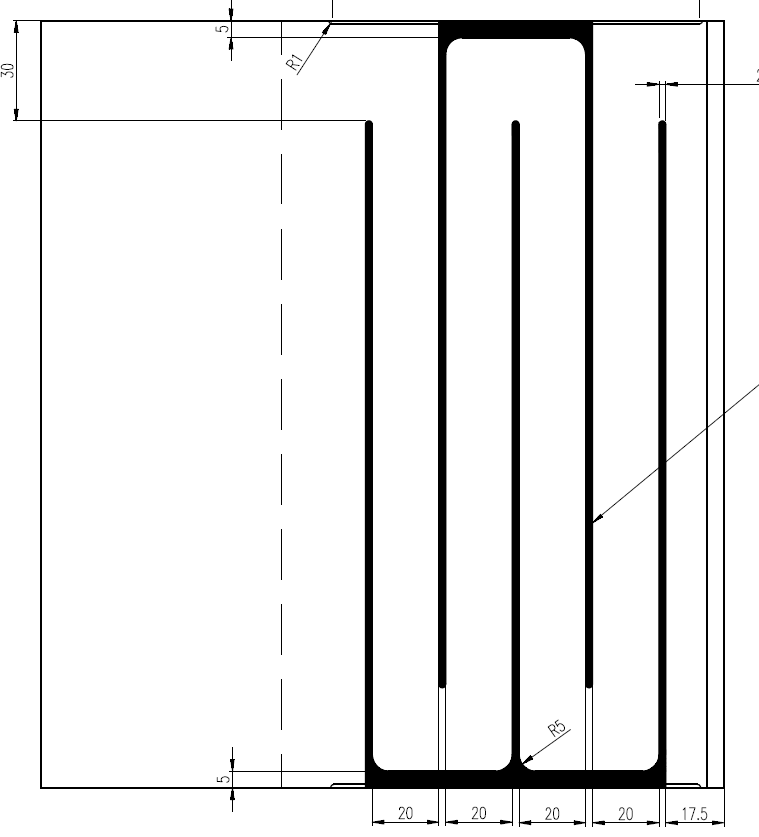
\includegraphics[width=0.4\textwidth]{Beam_Coupling_Impedance_Reduction_Techniques/figures/mke-serigraphy-diagram.png}
\label{fig:mke_layout}
}
\subfigure[]{
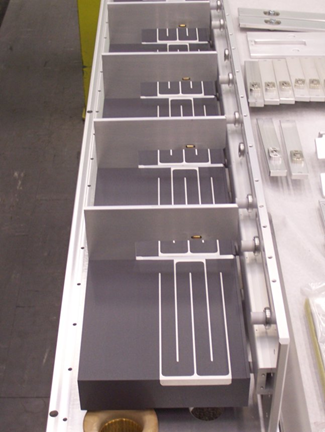
\includegraphics[width=0.4\textwidth]{Beam_Coupling_Impedance_Reduction_Techniques/figures/mke-serigraphy.png}
\label{fig:mke_picture}
}
\begin{center}
\subfigure[]{
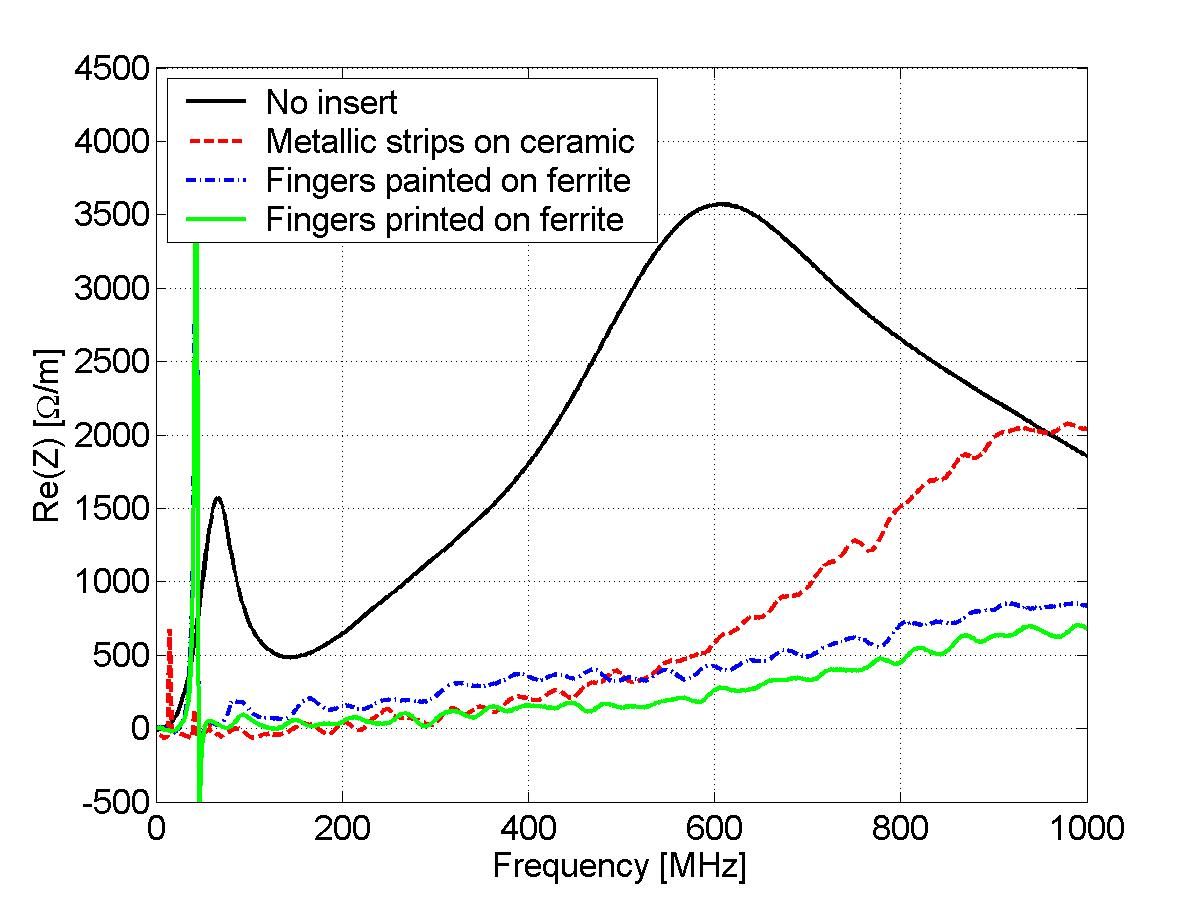
\includegraphics[width=0.4\textwidth]{Beam_Coupling_Impedance_Reduction_Techniques/figures/Printed_comparison_paper.jpg}
\label{fig:mke_impedance}
}
\end{center}
\caption{An example of seriagraphy in the SPS Extraction Kicker Magnets (SPS-MKE). The layout of the interleaved fingers is shown in \ref{fig:mke_layout} and the actual seriagraphed magnets in \ref{fig:mke_picture}. A comparison of the longitudinal beam coupling impedance with and without the seriagraphy is shown in \ref{fig:mke_impedance}.}
\label{fig:mke_figures}
\end{figure}

